\documentclass[pdflatex,iicol,sn-mathphys-num]{sn-jnl}
\usepackage{graphicx,xurl}
\usepackage{amsmath,amssymb,booktabs,array,tabularx,microtype,placeins,balance,tikz,capt-of}
\usetikzlibrary{arrows.meta}
\providecommand{\burl}[1]{\url{#1}}
\hypersetup{pdftitle={Adaptive Transfer Learning for Cold-Start Electric Vehicle Charging Demand Forecasting},pdfauthor={AIP491 G10 Research Team}}
\raggedbottom
\begin{document}
\title[Adaptive transfer learning]{Adaptive Transfer Learning for Cold-Start Electric Vehicle Charging Demand Forecasting}
\author{AIP491\_G10 Research Team}
\abstract{Forecasting charging demand at a location with little recorded history requires balancing source knowledge and local adaptation. We study 24-hour energy forecasting from the preceding 24 hours, with initial target histories of 7, 14 or 28 days. Independent small-scale benchmarks compare classical and neural models, while a separate GRU experiment calibrates target-only training before assessing transfer. Source initialization lowers Development MAE by 29.8--33.4\% relative to the calibrated target-only models. We then combine a source-retaining GRU and a recent-window GRU using delayed-loss Fixed-share weighting. On a previously inspected historical cohort spanning seven dataset namespaces, 90 selected entities and three random seeds, this adaptive mixture improves on the single Fixed-retention model in 18 of 21 namespace--history groups. A matched static mixture also improves in 18 groups. Adaptive weighting improves on that static mixture in 12 groups and worsens nine; all three UrbanEV groups remain worse than single Fixed retention. These results support transfer and complementary adaptation trajectories, with small and conditional additional benefits from online weighting. They do not establish a superior continuous-lambda controller or generalization to an untouched test set.}
\keywords{EV charging demand, cold start, transfer learning, GRU, retention regularization, online expert weighting}
\maketitle

\section{Introduction}
Charging locations with short observation histories offer few complete examples for a forecasting model. Training only on that local prefix can be unreliable, whereas a model pretrained on established locations may provide a useful starting point. UrbanEV and CHARGED offer hourly charging series for investigating this setting \cite{urbanev2025,charged2025}.

Our cold-start setting is operationally defined as \emph{limited recorded target history}: 7, 14 or 28 days before a replay begins. It is simulated on existing dataset identifiers, rather than verified physical opening dates. The forecasting task is unchanged throughout: the preceding 24 hourly bins predict the next 24 hourly energy values.

The central question is how source knowledge should influence subsequent adaptation. Three distinct mechanisms must be separated. Source initialization transfers model parameters. Retention regularization constrains departure from the source representation. An online decision rule changes how available predictors contribute to the deployed forecast. A gain from one mechanism is not evidence that another mechanism is effective.

We investigate three questions: (i) whether source initialization helps after strengthening target-only training; (ii) whether GRU is a reasonable compact backbone among the tested alternatives; and (iii) whether online weighting adds value beyond fixed retention and a static mixture of the same experts. The proposed forecasting system uses a standard GRU and an established expert-weighting rule. Its empirical contribution is the comparison of these mechanisms under delayed daily feedback, including unfavorable outcomes. The evidence remains exploratory because calibration and historical outcomes have prior exposure.

\section{Related work}
GRUs use gating to encode sequential observations \cite{cho2014}. We implement the standard PyTorch recurrence \cite{pytorch211}, without changing GRU layers or gates.

Transfer regularization can explicitly favor a pretrained solution. For example, $L^2$-SP penalizes parameter displacement from a pretrained reference \cite{li2018}. Our primary retention penalty instead compares normalized latent representations. The normalization and EV forecasting protocol are project-specific choices, not results established by that paper.

Continuous regularization coefficients can be adjusted through validation hypergradients \cite{luketina2016}. This motivates a separate lambda-only diagnostic. The mixture studied here instead changes forecast weights while each expert retains a constant regularization coefficient.

The historical retention selector uses paired errors and block bootstrap evidence, motivated by resampling methods for dependent observations \cite{kunsch1989}. The current mixture instead applies the Fixed-share expert rule \cite{herbster1998} to two adaptive GRU trajectories. We use its share-to-other update explicitly. We do not claim the original regret guarantees for unbounded energy losses and jointly trained recurrent models.

\section{Problem and data protocol}
\subsection{Inputs, targets and availability}
For target entity $i$ at daily origin $t$, the historical input is $X_{i,t}\in\mathbb R^{24\times7}$. Its channels are scaled energy, sine and cosine of hour, sine and cosine of weekday, weekend status and an observation mask. A separate $C_{i,t}\in\mathbb R^{24\times5}$ supplies the known future calendar channels. Weather and future energy are excluded. Recorded zeros are distinguished from missing historical values by the mask.

A positive energy scale $c_i$ is fitted only from the permitted target prefix and remains fixed during replay. Training labels are $y/c_i$; reported forecasts and errors are in kWh. Missing target labels are never filled. Scoring and updates require all 24 labels of a daily target vector to be available. An incomplete day updates neither the models nor the mixture weights.

At an origin, eligible earlier feedback is processed before issuing the current forecast. The current 24-hour forecast is persisted before its own labels can enter any update. Ninety daily origins are scheduled, but missing targets can reduce the number of scored days. If the initial prefix contains no complete examples, initialization keeps the Source weights and performs zero target optimizer steps.

\subsection{Experimental cohorts}
\begin{table*}[t]
\centering\small
\caption{Distinct experimental cohorts and training recipes.}\label{tab:scope}
\begin{tabularx}{\textwidth}{@{}>{\raggedright\arraybackslash}p{.19\textwidth}>{\raggedright\arraybackslash}p{.28\textwidth}>{\raggedright\arraybackslash}p{.12\textwidth}>{\raggedright\arraybackslash}X@{}}\toprule
Study & Target scope & Initial history & Source and purpose\\\midrule
Independent baselines & 4 UrbanEV Development entities; two implementations & 14 days & Source trained for 3 epochs per neural backbone; architecture and initialization comparisons\\
Calibrated GRU & 4 calibration entities; 12 additional Development entities for evaluation & 7 / 14 / 28 days & Reused Source epoch 10; initial-epoch calibration, transfer and retention comparisons\\
Historical follow-up & 30 UrbanEV entities; 10 in each of 6 CHARGED namespaces & 7 / 14 / 28 days & Namespace-specific Source epoch 10; fixed-recipe stable/fast mixture comparison\\
\bottomrule\end{tabularx}
\end{table*}

Table~\ref{tab:scope} separates the three evidence streams. The four benchmark/calibration IDs are 1405, 2152, 1153 and 1693. Their 14-day prefixes contain 4, 12, 13 and 13 complete examples, respectively. Both baseline implementations use 65,888 eligible Source examples but train their neural Source models independently.

Twelve additional Development entities are selected to balance four prefix zero-fraction strata. Each history budget provides 888 scored entity-days per seed, with 51--90 complete scored days per entity.

The historical follow-up comprises UrbanEV/SZH and CHARGED/AMS, JHB, LOA, MEL, SPO and SZH. Source pretraining and target adaptation remain within each dataset namespace; there is no joint cross-city Source model. Seven namespaces times three history budgets give 21 groups, not 21 cities. Ninety selected entities times three budgets times seeds 42, 43 and 44 give 810 units. UrbanEV ID 2193 is unscored in all nine of its units and remains explicit in coverage. The matrix contains 67,293 scored entity--history--seed days.

Source and target IDs are disjoint in the prepared split. This is an identifier-level statement, not proof of distinct physical sites across datasets. The historical cohort reuses previously inspected Final entities and dates; it is a historical follow-up, not a new untouched Final evaluation. No absolute MAE is pooled across these different studies or namespaces.

\section{Forecasting method}
\subsection{GRU encoder and prediction head}
\begin{figure*}[t]
\centering
\definecolor{FlowBlue}{HTML}{2166AC}
\definecolor{FlowRed}{HTML}{B2182B}
\begin{tikzpicture}[x=1.12cm,y=0.79cm,>=Latex,
  every node/.style={font=\footnotesize,align=center},
  box/.style={draw=black!35,rounded corners=2pt,fill=white,line width=.6pt,inner sep=7pt},
  flow/.style={->,line width=.75pt,draw=black!65},
  ref/.style={->,dashed,line width=.75pt,draw=FlowBlue}]
\node[box,text width=7.2cm,minimum height=.95cm,draw=FlowBlue!60,fill=FlowBlue!7] (source) at (7,9)
 {\textbf{Source pretraining}\\[-1pt]Established entities in one namespace $\rightarrow$ GRU checkpoint $\theta_s$ and latent scales $s$};
\node[box,text width=4.0cm,minimum height=.9cm] (input) at (7,7)
 {\textbf{Permitted target inputs}\\[-1pt]$X_t\in\mathbb R^{24\times7}$, $C_t\in\mathbb R^{24\times5}$};
\node[box,text width=5.0cm,minimum height=1.35cm,draw=FlowBlue!65,fill=FlowBlue!9] (stable) at (3.8,4.7)
 {\textbf{Stable expert}\\[2pt]GRU encoder + calendar head\\$\lambda_S=1$, $L_S=F+R$\\Newly arrived day};
\node[box,text width=5.0cm,minimum height=1.35cm,draw=FlowRed!60,fill=FlowRed!7] (fast) at (10.2,4.7)
 {\textbf{Fast expert}\\[2pt]GRU encoder + calendar head\\$\lambda_F=0$, $L_F=F$\\Last 7 calendar days};
\node[box,text width=5.0cm,minimum height=.85cm,draw=FlowBlue!65,fill=FlowBlue!9] (mix) at (7,2.5)
 {\textbf{Adaptive forecast mixture}\\$\hat y_t=w_t\hat y_{S,t}+(1-w_t)\hat y_{F,t}$};
\node[font=\small] (out) at (7,.9) {\textbf{Persist the next 24-hour energy forecast}\\[-1pt]No future energy labels enter this prediction};
\draw[flow] ([xshift=-3.584cm]source.south) -- (stable.north);
\draw[flow] ([xshift=3.584cm]source.south) -- (fast.north);
\node[fill=white,font=\footnotesize,inner sep=2pt] at (3.8,7.8) {initialize};
\node[fill=white,font=\footnotesize,inner sep=2pt] at (10.2,7.8) {initialize};
\draw[flow] (input.south) -- (7,6.1) -| ([xshift=1.4cm]stable.north);
\draw[flow] (7,6.1) -| ([xshift=-1.4cm]fast.north);
\draw[ref] (source.west) -- (.5,9) -- (.5,4.7) -- (stable.west);
\node[fill=white,text width=1.1cm,font=\footnotesize,inner sep=2pt] at (.5,6.8) {frozen\\reference\\for $R$};
\draw[flow] (stable.south) -- (3.8,2.5) -- (mix.west);
\draw[flow] (fast.south) -- (10.2,2.5) -- (mix.east);
\node[fill=white,font=\footnotesize,inner sep=2pt] at (3.8,3.2) {$\hat y_{S,t}$};
\node[fill=white,font=\footnotesize,inner sep=2pt] at (10.2,3.2) {$\hat y_{F,t}$};
\draw[flow] (mix.south) -- (out.north);
\end{tikzpicture}

\caption{Source transfer, retention and the two-expert forecast.}\label{fig:model}
\end{figure*}

Figure~\ref{fig:model} distinguishes parameter initialization from the frozen reference used in retention. Both target experts receive the permitted historical and future-calendar inputs. The mixture combines their forecasts with complementary weights $w$ and $1-w$.

The encoder has two GRU layers with hidden width 64 and zero dropout. Using within-window step $\tau$, the recurrence is
\begingroup\small
\begin{equation}\begin{aligned}
r_\tau&=\sigma(W_{ir}x_\tau+b_{ir}+W_{hr}h_{\tau-1}+b_{hr}),\\
z_\tau&=\sigma(W_{iz}x_\tau+b_{iz}+W_{hz}h_{\tau-1}+b_{hz}),
\end{aligned}\label{eq:gates}\end{equation}
\endgroup
\begin{equation}\begin{aligned}
n_\tau&=\tanh\!\left(W_{in}x_\tau+b_{in}\right.\\
&\qquad\left.+r_\tau\odot(W_{hn}h_{\tau-1}+b_{hn})\right),\\
h_\tau&=(1-z_\tau)\odot n_\tau+z_\tau\odot h_{\tau-1}.
\end{aligned}\label{eq:hidden}\end{equation}
These are the PyTorch gate conventions \cite{pytorch211}; in particular, the reset gate is applied after the recurrent affine transformation in the candidate state. Hidden state is reset for each input window and is not passed between entities.

The last-layer final state $h_{24}\in\mathbb R^{64}$ is concatenated with the 120 flattened future-calendar values. The head applies a width-64 linear layer, ReLU, a 24-output linear layer and Softplus. The primary forecaster has 52,376 trainable parameters. A same-width, two-layer LSTM with this head would have 65,368; this is a parameter-count comparison, not a measured speed or accuracy advantage.

\subsection{Forecast loss and latent retention}
Let $B$ be a batch of complete examples for one target, and let $\widetilde y$ and $\widehat{\widetilde y}$ denote normalized labels and predictions. Forecast training uses
\begin{equation}
F_B(\theta)=\frac{1}{24|B|}\sum_{j\in B}\sum_{q=1}^{24}
\left|\widehat{\widetilde y}_{j,q}(\theta)-\widetilde y_{j,q}\right|.
\label{eq:forecastloss}\end{equation}
Let $h(x;\theta_s)$ be the frozen Source encoder output and $s_k$ the population standard deviation of its $k$th latent coordinate on the permitted Source training population. The retention term is
\begin{equation}\begin{aligned}
R_B(\theta)&=\frac{1}{64|B|}\sum_{j\in B}\sum_{k=1}^{64}u_{j,k}^{2},\\
u_{j,k}&=\frac{h_k(x_j;\theta)-h_k(x_j;\theta_s)}{s_k+\epsilon_R}.
\end{aligned}\label{eq:retention}\end{equation}
with $\epsilon_R=0.001$. The reference and scales receive no target gradients. Division occurs before squaring. The total target objective is
\begin{equation}
L_B(\theta,\lambda)=F_B(\theta)+\lambda R_B(\theta).
\label{eq:total}\end{equation}
A separate 21-coefficient diagnostic search included lambda values up to 33.844, but does not define universal retention regimes. Lambda controls an explicit representation penalty; it is neither the optimizer learning rate nor a percentage of retained knowledge. Setting lambda to zero removes the penalty while preserving transferred initialization.

\subsection{Stable and fast adaptation trajectories}
The stable expert is the historical Fixed model: Source epoch-10 initialization, fixed $\lambda_S=1$, three initial target epochs when complete prefix examples exist, Adam learning rate 0.001, and one online epoch on each newly arrived complete daily example. Its authenticated saved forecasts are reused.

The fast expert starts from the matching Source weights but uses fixed $\lambda_F=0$. It has the same three initial epochs and Adam learning rate. At each complete arrival, it trains for one epoch on available examples within the seven calendar days ending at the arrived example's forecast origin. The window can include permitted prefix examples, contains at most seven complete daily examples and fits one optimizer step. It never includes future labels.

The experts have the same architecture but different adaptation objectives and memory. The source reference stays frozen while target model parameters adapt. The mixture controller changes forecast weights; both expert lambda coefficients remain constant.

\subsection{Adaptive forecast weighting}
Let $w_t$ be the current stable-expert weight. The 24-dimensional forecast in original energy units is
\begin{equation}
\hat y_{t,q}=w_t\hat y_{S,t,q}+(1-w_t)\hat y_{F,t,q}.
\label{eq:mixture}\end{equation}
For an earlier issued day $d$ whose complete labels have arrived, each expert's saved forecast supplies normalized loss
\begin{equation}
\ell_{e,d}=\frac{1}{24c_i}\sum_{q=1}^{24}|\hat y_{e,d,q}-y_{d,q}|,
\quad e\in\{S,F\}.
\label{eq:feedbackloss}\end{equation}
Use feedback-event index $k$ separately from forecast-origin index $t$. The exponential loss posterior is
\begin{equation}
p_k=\frac{w_k e^{-\eta\ell_{S,d}}}
{w_k e^{-\eta\ell_{S,d}}+(1-w_k)e^{-\eta\ell_{F,d}}}.
\label{eq:posterior}\end{equation}
The two-expert share-to-other step \cite{herbster1998} is
\begin{equation}
w_{k+1}=(1-\alpha)p_k+\alpha(1-p_k)
=\alpha+(1-2\alpha)p_k.
\label{eq:share}\end{equation}
The implementation uses equivalent log-odds arithmetic for numerical stability. Calibration selected $w_0\approx0.4308$, $\eta=0.1$ and $\alpha=0.1$. Consequently updated weights lie in $[0.1,0.9]$. This interval is a consequence of the selected share coefficient, not a searched lambda range or proof of an optimal weight domain.

\begin{figure*}[t]
\centering
\definecolor{FlowBlue}{HTML}{2166AC}
\definecolor{FlowRed}{HTML}{B2182B}
\begin{tikzpicture}[x=1.10cm,y=.95cm,>=Latex,
  every node/.style={font=\footnotesize,align=center},
  box/.style={draw=black!35,rounded corners=2pt,fill=white,line width=.6pt,inner sep=6pt,text width=3.1cm,minimum height=1.1cm},
  flow/.style={->,line width=.75pt,draw=black!65}]
\node[box,draw=FlowRed!55,fill=FlowRed!7] (labels) at (1.5,2.8) {\textbf{Arrived labels}\\Complete earlier day $d$};
\node[box,draw=FlowBlue!55,fill=FlowBlue!5] (saved) at (1.5,.4) {\textbf{Saved forecasts}\\$\hat y_{S,d},\hat y_{F,d}$\\Issued before $y_d$};
\node[box] (train) at (5.3,2.8) {\textbf{Expert updates}\\Stable: one new day\\Fast: recent window};
\node[box,draw=FlowRed!45,fill=FlowRed!4] (loss) at (5.3,.4) {\textbf{Expert losses}\\Normalized daily MAE\\$\ell_{S,d},\ell_{F,d}$};
\node[box,draw=FlowBlue!65,fill=FlowBlue!9] (weights) at (9,.4) {\textbf{Weight update}\\Posterior $p_k$\\Fixed-share $w_{k+1}$};
\node[box,draw=FlowBlue!65,fill=FlowBlue!9] (next) at (12.7,2.8) {\textbf{Current forecast}\\Updated models and $w$\\After eligible feedback};
\draw[flow] (labels.east) -- (train.west);
\draw[flow] (labels.south) -- (1.5,1.55) -- (5.3,1.55) -- (loss.north);
\draw[flow] (saved.east) -- (loss.west);
\draw[flow] (loss.east) -- (weights.west);
\draw[flow] (train.east) -- (next.west);
\draw[flow] (weights.east) -- (12.7,.4) -- (next.south);
\end{tikzpicture}

\caption{Causal processing of complete daily feedback.}\label{fig:feedback}
\end{figure*}

Figure~\ref{fig:feedback} shows observed labels as an independent input, separate from saved predictions. At each origin, earlier feedback is processed in label-availability order and then origin order. Both experts are updated from eligible observations, and the mixture weight is updated from their \emph{saved pre-update forecasts}. The current forecast is then issued. Missing days produce no weighting event; elapsed time alone does not decay weights. This is soft forecast fusion, not winner-take-all model switching or continuous lambda adaptation.

\section{Experimental design}
\subsection{Calibration and comparators}
The independent baseline studies each contain 172 unique model--mode--entity--seed rows: 160 nonspatial and 12 spatial. Deterministic methods are not replicated with artificial seeds. Neural Source training uses three epochs. Target adaptation uses three epochs, batch size four and learning rate 0.0005, followed by one online epoch per eligible arrival. Implementation-specific architecture and tokenization differences remain explicit.

For the calibrated GRU study, initial epoch candidates are 3, 10, 30, 100 and 300. Selection minimizes equal-entity, equal-seed MAE on the first 28 scheduled calibration origins of the four calibration entities. A declared extension to 900 epochs is unused because no 300-epoch candidate wins. The selected target-only epochs are 30/100/100 for 7/14/28-day histories; Source-initialized models select 3/3/10. Learning rate is 0.001. The additional twelve entities evaluate the selected recipes.

This study's independent retention bank uses $\lambda\in\{0,0.1,1\}$. Fixed selection chooses 1/1/0 across the three history budgets. Past-MAE selection and confidence selection receive the same three independent trajectories and start from the calibration-selected expert. The confidence gate uses a seven-day block, at least five complete days, moving segments of length three, 2,000 bootstrap resamples, a 0.05 interval parameter and zero required margin. These three lambda candidates are a historical comparator bank, not a newly justified universal set of retention regimes.

For the stable/fast mixture, four UrbanEV calibration entities and seeds 42--44 compare fast windows of 3, 7 and 14 days with learning rates 0.001 and 0.003. Each pair receives a static stable weight minimizing equal-cell calibration MAE on $[0,1]$ via the weighted-median solution of the convex absolute-error objective. The selected seven-day, 0.001 recipe determines $w_0$.

Nine subsequent controller candidates cross $\eta\in\{0.1,1,10\}$ and $\alpha\in\{0.001,0.01,0.1\}$. Calibration selects the settings above. These bounded engineering grids do not establish global optima. The resulting recipe is carried unchanged into all seven namespaces and all three history budgets; the historical follow-up performs no per-namespace recalibration.

The original historical selector reforks model and optimizer states every 14 days. Seven-day readbacks of its archived forecasts are shadow-selection diagnostics, not newly executed seven-day reforked training. The essential comparators are single Fixed retention, the historical confidence selector, Fast-only, and a static mixture with the \emph{same two expert forecasts and initial weight}. Equal-weight and loss-free sharing mixtures are additional posthoc controls. In loss-free sharing, the posterior is set equal to the prior before applying the same share step, removing loss feedback but retaining the pull toward one-half.

\subsection{Metrics and aggregation}
For complete scored origins $\mathcal D_{i,s}$ of entity $i$ and seed $s$, define
\begin{equation}
\operatorname{MAE}_{i,s}=\frac{1}{24|\mathcal D_{i,s}|}
\sum_{d\in\mathcal D_{i,s}}\sum_{q=1}^{24}|\hat y_{i,s,d,q}-y_{i,d,q}|.
\label{eq:metric}\end{equation}
All compared methods share the same scored origins within a unit. Group MAE first averages seeds within each entity and then averages scored entities equally within one namespace--history group. Unscored entities remain null; they are not assigned zero error. We do not pool hourly records across entities or pool kWh errors across namespaces with different scales.

For a named reference $A$ and candidate $B$, the reported reduction is $100(\operatorname{MAE}_A-\operatorname{MAE}_B)/\operatorname{MAE}_A$. Positive values indicate lower error. Table minima are bold at printed precision; displayed ties receive equal emphasis. The 21 group means share entities and dates, so their win counts are descriptive, not 21 independent trials or a significance test.

\section{Results}
\subsection{Backbone and transfer comparisons}
\begin{table*}[t]
\centering\small
\caption{Independent baseline MAE (kWh; lower is better).}\label{tab:baselines}
\begin{tabular*}{\textwidth}{@{\extracolsep{\fill}}lrrrr@{}}\toprule
& \multicolumn{2}{c}{Implementation A} & \multicolumn{2}{c}{Implementation B}\\\cmidrule(lr){2-3}\cmidrule(l){4-5}
Model & Target only & Transfer & Target only & Transfer\\\midrule
Daily naive & 7.0763 & -- & 7.0757 & --\\
Weekly naive & 8.4631 & -- & 8.4631 & --\\
Ridge & 5.9339 & -- & 5.9339 & --\\
SARIMA & 6.5799 & -- & 6.6771 & --\\
Random forest & \textbf{5.8008} & -- & \textbf{5.8204} & --\\
XGBoost & 6.4847 & -- & 6.4613 & --\\
MLP & 8.6711 & 5.5196 & 8.6855 & 5.4753\\
GRU & 8.9406 & \textbf{5.3150} & 8.9239 & 5.3157\\
LSTM & 8.9360 & 5.3356 & 8.9565 & 5.3168\\
TCN & 8.0734 & 5.3447 & 7.8415 & 5.3027\\
Custom attention & 8.1209 & 5.5823 & -- & --\\
Official TimeXer & -- & -- & 7.0224 & \textbf{5.1979}\\
GCN--LSTM (spatial) & 7.1288 & -- & 7.1790 & --\\
\bottomrule\end{tabular*}
\end{table*}

Table~\ref{tab:baselines} bolds the lowest value in each implementation/training-mode column. A dash means that mode is not reported for that model; it is not a zero result. Spatial GCN--LSTM additionally receives support histories, so its information set differs from the nonspatial rows.



The paired visualization in Appendix~\ref{app:backbones} compares initialization modes separately within each implementation. All 60 paired neural entity--seed comparisons in each implementation favor Source initialization. Among transferred models, A's GRU has MAE 5.3150, ahead of LSTM 5.3356 and TCN 5.3447. In B, the official TimeXer adapter \cite{wang2024timexer} has the lowest MAE, 5.1979, compared with GRU 5.3157. A's custom attention adapter omits the reference TimeXer patch/global-token construction; it is not an architecture-matched replication of B's official adapter.

These fixed-recipe, four-entity results support GRU as a competitive controlled backbone with a compact established implementation. They do not prove GRU is universally best, and they are not pooled into a shared ranking. Source3 baseline results and Source10 retention results also remain separate.

\subsection{Transfer after target-only calibration}
\begin{table}[t]
\centering\small
\caption{Twelve-entity Development MAE (kWh).}\label{tab:history}
\begin{tabularx}{\columnwidth}{@{}>{\raggedright\arraybackslash}Xrrr@{}}\toprule
Method & 7 days & 14 days & 28 days\\\midrule
Daily naive & 5.0906 & 5.0906 & 5.0906\\
Weekly naive & 6.0773 & 6.0773 & 6.0773\\
Target only & 5.0521 & 4.8341 & 4.7697\\
Source fine-tune & 3.3671 & 3.3046 & 3.3482\\
Fixed & \textbf{3.3186} & \textbf{3.2670} & 3.3482\\
Past MAE & 3.3234 & 3.2904 & 3.3252\\
Confidence gate & 3.3234 & 3.2755 & \textbf{3.3140}\\
\bottomrule\end{tabularx}
\end{table}

Table~\ref{tab:history} reports equal-entity MAE, with minima bold within each history column. Source fine-tuning lowers MAE relative to calibrated target-only training by 33.35\%, 31.64\% and 29.80\% at 7, 14 and 28 days. The transfer benefit persists after the target-only initial training budget is calibrated.

Retention and selection gains are much smaller. Fixed has the lowest MAE at 7 and 14 days; confidence selection has the lowest reported value at 28 days. There it beats the calibration-selected Fixed by 1.02\%, but that Fixed selected lambda zero. A retrospectively selected lambda-one constant gives 3.2925 kWh, below confidence selection's 3.3140. This retrospective value is a diagnostic using evaluated labels, not an admissible replacement for calibration selection. The result does not establish general superiority of confidence gating.

\subsection{Complete historical-cohort comparison}


Table~\ref{tab:cohort} includes both component experts and both mixture rules; bold marks the best of the five listed methods in each row. Fixed uses lambda one. Fast-only uses lambda zero and the seven-day update window. Static and adaptive mixtures share exactly these expert forecasts. This comparison separates the two-expert family from the incremental effect of changing its weights.

The adaptive mixture has lower MAE than single Fixed in 18 of 21 groups; the original selector wins 9 of 21 and Fast-only wins 16 of 21. All 18 CHARGED groups improve under the adaptive mixture, by 0.23--7.77\%. All three UrbanEV groups worsen, by 0.88\%, 0.32\% and 0.45\%. A static mixture also wins 18 of 21 against single Fixed. Thus the expanded win count alone cannot establish that adaptive weighting causes the improvement.

\begin{figure*}[t]
\centering
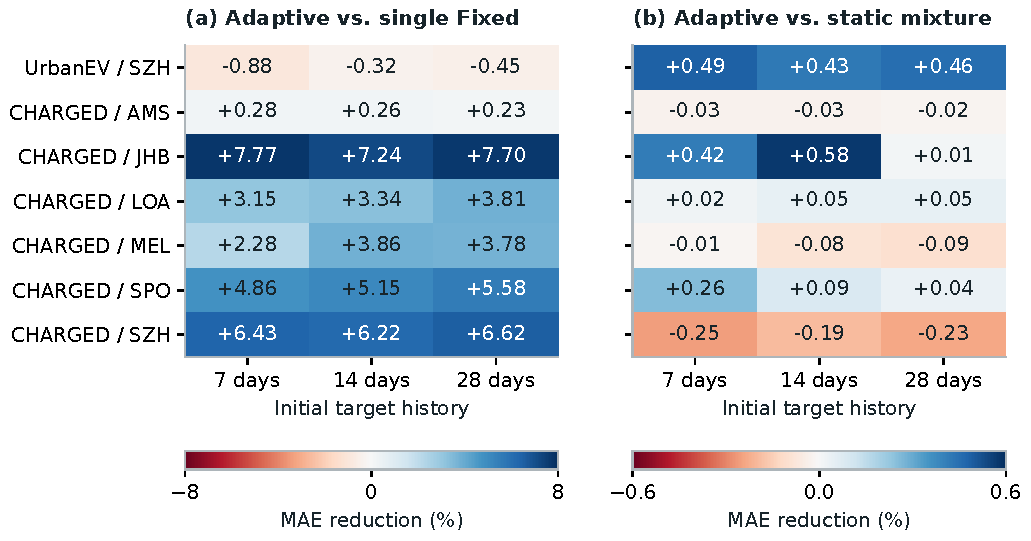
\includegraphics[width=\textwidth]{figures/cohort-comparisons.pdf}
\caption{Mixture gains and the incremental weighting effect.}\label{fig:cohort}
\end{figure*}

Figure~\ref{fig:cohort} names the denominator in each panel. The left panel measures the combined mixture-family benefit against single Fixed; the right measures only the additional benefit against the same static mixture. Their color scales differ explicitly because these effects have different magnitudes. Positive values indicate improvement in both panels.

Adaptive weighting improves on the static mixture in 12 groups and worsens nine. UrbanEV, JHB, LOA and SPO favor adaptive weights at all three histories; AMS, MEL and CHARGED/SZH favor static weights. Even where weighting improves the UrbanEV mixture, it does not recover the stronger single Fixed result. Against the original selector, the adaptive mixture improves in 20 groups and worsens one, UrbanEV at seven days.

\begin{table}[t]
\centering\small
\setlength{\tabcolsep}{3pt}
\caption{Adaptive gains against fusion controls.}\label{tab:controls}
\begin{tabularx}{\columnwidth}{@{}>{\raggedright\arraybackslash}Xrrr@{}}\toprule
Reference & Wins & Min (\%) & Max (\%)\\\midrule
Calibrated static & 12 / 21 & $-0.250$ & $+0.580$\\
Equal 50/50 & 21 / 21 & $+0.00084$ & $+0.263$\\
Loss-free sharing & 21 / 21 & $+0.00097$ & $+0.227$\\
\bottomrule\end{tabularx}
\end{table}

Table~\ref{tab:controls} counts groups in which adaptive mixing is lower than each reference; the range is its percentage reduction across all groups. Equal weighting and loss-free sharing are posthoc diagnostics, with no new training or parameter selection. Their positive signs suggest a small additional role for loss feedback on these inspected data, but do not establish statistical significance, a large controller effect or independent confirmation.

Recorded temporal examples and their fixed selection rule are provided in Appendix~\ref{app:traces}.

\FloatBarrier
\section{Discussion and limitations}
The static control shows that improvement over single Fixed combines complementary experts with a smaller weighting effect. The 18/21 mixture-family win count therefore does not isolate adaptive control.

All cohorts have prior exposure. The baseline recipes are untuned and partly architecture-specific; they do not establish GRU optimality. Identifier-level splits do not certify physical independence across datasets.

The controller changes forecast weights, not lambda. A separate four-target later-window Adam hypergradient diagnostic gave MAE 4.806223 versus calibrated Fixed 4.803054. A persistent lambda-only controller also failed its Calibration promotion threshold. Neither diagnostic is the mixture experiment.

Two trajectories, different update memories and GPU/CPU execution have different costs. Total pretraining, exploration and end-to-end resources were not jointly measured, so equal-cost superiority is unestablished. Errors were reconstructed on common masks with nine null units preserved. Baseline A received an independent artifact readback; B reuses a published readback on unchanged ledgers. Full training reproduction, physical issuance chronology, every historical bootstrap resample and fresh publisher-archive authentication remain unverified here.

Confirmatory claims require an untouched cohort or prospective period, a separately registered evaluation and fuller compute accounting.

\section{Conclusion}
Source-initialized GRU remains competitive and lowers MAE after target-only training is calibrated. Across historical groups, both adaptive and static mixtures beat single Fixed in 18/21. Adaptive weights improve on static in 12/21 and worsen nine; all three UrbanEV groups remain worse than Fixed. The evidence supports complementary experts and conditional weighting benefits, with independent confirmation still needed.

\FloatBarrier
\clearpage
\onecolumn
\appendix
\section{Complete historical comparison}\label{app:cohort}
Table~\ref{tab:cohort} retains all 21 groups and both single-expert and mixture methods. Minima are bold within each row at displayed precision. The nine unscored units remain in the underlying coverage ledger.

\noindent\begin{minipage}{\textwidth}
\centering\small
\captionof{table}{Historical-cohort MAE for all 21 groups (kWh).}\label{tab:cohort}
\begin{tabular*}{\textwidth}{@{\extracolsep{\fill}}lrrrrrr@{}}\toprule
Namespace & Days & Fixed & Original selector & Fast-only & Static mix & Adaptive mix\\\midrule
UrbanEV / SZH & 7 & \textbf{8.0400} & 8.1014 & 8.5260 & 8.1510 & 8.1111\\
UrbanEV / SZH & 14 & \textbf{7.9758} & 8.0517 & 8.3709 & 8.0361 & 8.0016\\
UrbanEV / SZH & 28 & \textbf{7.9159} & 8.0015 & 8.3353 & 7.9879 & 7.9512\\
\addlinespace[3pt]
CHARGED / AMS & 7 & 6.1483 & 6.1559 & \textbf{6.1272} & 6.1294 & 6.1310\\
CHARGED / AMS & 14 & 6.1482 & 6.1520 & \textbf{6.1281} & 6.1305 & 6.1321\\
CHARGED / AMS & 28 & 6.1482 & 6.1529 & 6.1334 & \textbf{6.1331} & 6.1343\\
\addlinespace[3pt]
CHARGED / JHB & 7 & 1.3206 & 1.3685 & 1.3231 & 1.2230 & \textbf{1.2179}\\
CHARGED / JHB & 14 & 1.3227 & 1.3604 & 1.3611 & 1.2341 & \textbf{1.2269}\\
CHARGED / JHB & 28 & 1.2919 & 1.3560 & 1.2632 & 1.1926 & \textbf{1.1924}\\
\addlinespace[3pt]
CHARGED / LOA & 7 & 1.3220 & 1.3273 & 1.3118 & 1.2807 & \textbf{1.2803}\\
CHARGED / LOA & 14 & 1.3334 & 1.3431 & 1.3272 & 1.2895 & \textbf{1.2889}\\
CHARGED / LOA & 28 & 1.3265 & 1.3271 & 1.3139 & 1.2765 & \textbf{1.2759}\\
\addlinespace[3pt]
CHARGED / MEL & 7 & 52.8482 & 52.1542 & 52.3596 & \textbf{51.6384} & 51.6443\\
CHARGED / MEL & 14 & 54.3655 & 53.0840 & 52.9679 & \textbf{52.2222} & 52.2649\\
CHARGED / MEL & 28 & 54.2423 & 53.0832 & 52.7780 & \textbf{52.1444} & 52.1934\\
\addlinespace[3pt]
CHARGED / SPO & 7 & 2.0217 & 1.9702 & 2.0017 & 1.9284 & \textbf{1.9234}\\
CHARGED / SPO & 14 & 1.9893 & 1.9414 & 1.9444 & 1.8887 & \textbf{1.8869}\\
CHARGED / SPO & 28 & 2.0256 & 1.9679 & 1.9707 & 1.9133 & \textbf{1.9126}\\
\addlinespace[3pt]
CHARGED / SZH & 7 & 91.8211 & 90.6306 & 87.3766 & \textbf{85.7026} & 85.9166\\
CHARGED / SZH & 14 & 90.8436 & 89.3300 & 86.8287 & \textbf{85.0301} & 85.1907\\
CHARGED / SZH & 28 & 90.8853 & 89.3310 & 86.3015 & \textbf{84.6675} & 84.8648\\
\bottomrule\end{tabular*}
\end{minipage}

\section{Paired backbone visualization}\label{app:backbones}
Figure~\ref{fig:backbones} visualizes the neural rows of Table~\ref{tab:baselines}. Each segment joins target-only and Source-initialized results within one implementation; the two panels share the numerical axis.

\noindent\begin{minipage}{\textwidth}
\centering
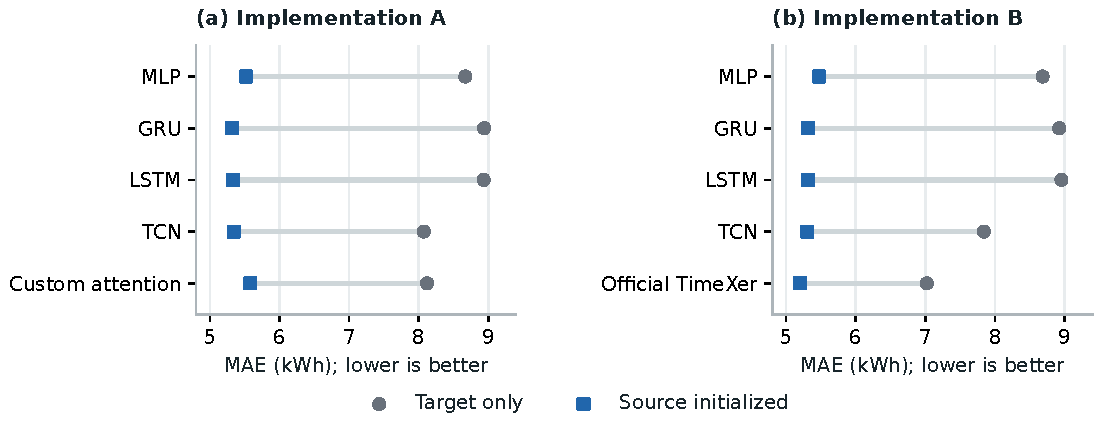
\includegraphics[width=.88\textwidth]{figures/backbones.pdf}
\captionof{figure}{Paired target-only and transferred neural backbones.}\label{fig:backbones}
\end{minipage}
\clearpage
\section{Recorded temporal examples}\label{app:traces}
The two 14-day-history examples use seed 42. Within JHB and UrbanEV separately, select the upper median of seed-averaged percentage gain among entities with Fixed MAE above $10^{-4}$ kWh. This selects JHB ID 13 and UrbanEV ID 1272. Figure~\ref{fig:traces} is descriptive: its individual signs need not match namespace means. Dates are forecast origins; errors accumulate over scored origins. Separate error axes retain each entity's energy scale.

\noindent\begin{minipage}{\textwidth}
\centering
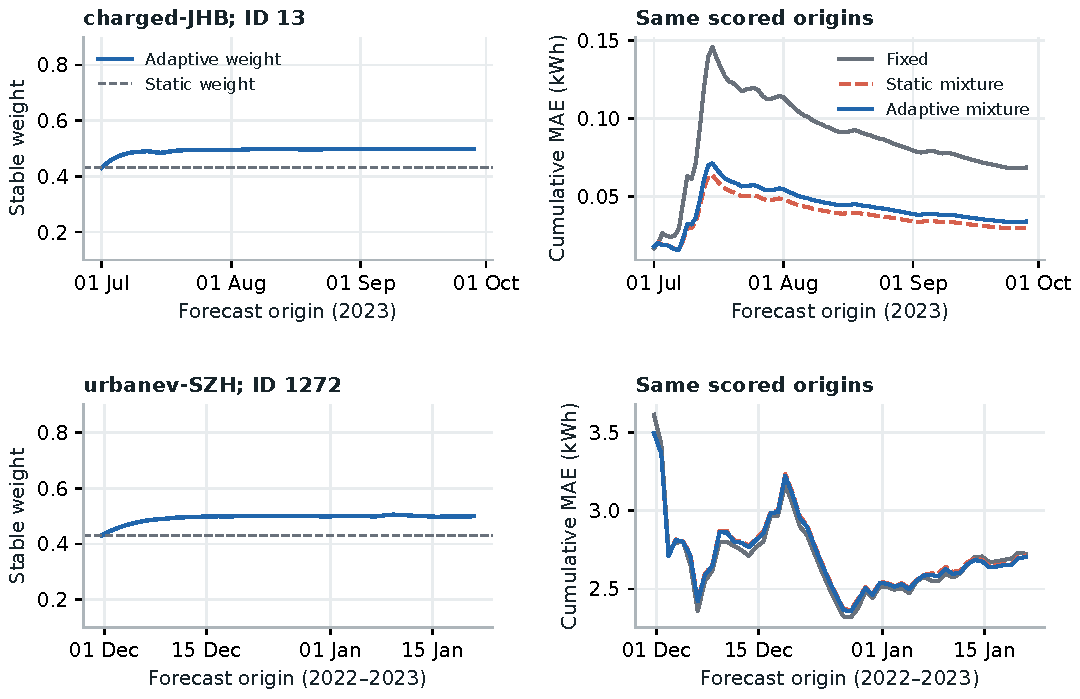
\includegraphics[width=.85\textwidth]{figures/trajectories.pdf}
\captionof{figure}{Weight trajectories and cumulative error examples.}\label{fig:traces}
\end{minipage}

\section{Initial-training calibration}\label{app:calibration}
Figure~\ref{fig:calibration} shows every registered candidate on a shared MAE scale. Stars mark selected candidates, not global optima. The four-entity calibration selects 30/100/100 target-only epochs and 3/3/10 Source-initialized epochs. The curves summarize four calibration entities; Table~\ref{tab:history} reports twelve-entity evaluation.

\noindent\begin{minipage}{\textwidth}
\centering
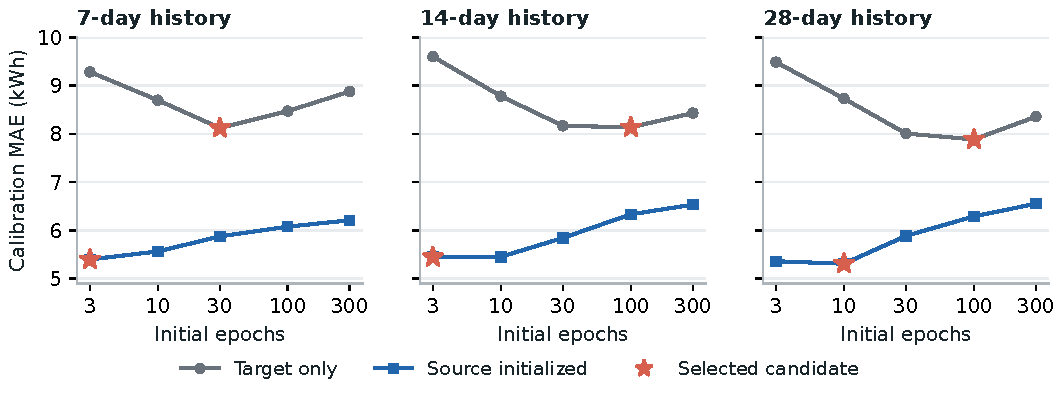
\includegraphics[width=.9\textwidth]{figures/calibration.pdf}
\captionof{figure}{Registered initial-epoch calibration curves.}\label{fig:calibration}
\end{minipage}

\clearpage
\twocolumn
\backmatter
\balance
\bibliography{references}
\end{document}
